% Đặc trưng

% Dưới đây là một số đặc điểm của một kiến trúc kiến trúc vi dịch vụ tốt:

% Mô - đun hóa : Kiến trúc nên bao gồm một tập hợp các dịch vụ được kết hợp lỏng lẻo có thể được triển khai, duy trì và mở rộng quy mô một cách độc lập.

% Triển khai độc lập : Mỗi dịch vụ phải có khả năng triển khai độc lập để có thể thực hiện các thay đổi đối với một dịch vụ mà không ảnh hưởng đến các dịch vụ khác.

% Bối cảnh giới hạn : Kiến trúc phải được thiết kế để phù hợp với ranh giới của khả năng kinh doanh, sao cho mỗi dịch vụ chịu trách nhiệm về một tập hợp chức năng cụ thể, gắn kết.

% Tự chủ : Các dịch vụ phải có khả năng hoạt động tự chủ, ít phụ thuộc vào các dịch vụ khác.

% Khả năng phục hồi : Kiến trúc phải được thiết kế để chịu đựng lỗi và các dịch vụ phải có khả năng xử lý lỗi một cách duyên dáng.

% Khả năng mở rộng : Kiến trúc phải được thiết kế để hỗ trợ mở rộng quy mô các dịch vụ riêng lẻ cũng như toàn bộ hệ thống.

% Tính linh hoạt : Kiến trúc phải cho phép phát triển và triển khai nhanh chóng các dịch vụ mới cũng như khả năng thay đổi các dịch vụ hiện có một cách nhanh chóng và dễ dàng.

% Văn hóa DevOps : Kiến trúc phải được hỗ trợ bởi văn hóa nhấn mạnh sự cộng tác và giao tiếp giữa các nhóm phát triển và vận hành, cũng như tự động hóa các quy trình triển khai và thử nghiệm.

Kiến trúc vi dịch vụ có nhiều ưu điểm đặc biệt với các dự án có quy mô lớn và phức tạp.

Kiến trúc vi dịch vụ phân chia dự án thành các dịch vụ nhỏ.

Giúp việc phát triển và quản lý dễ dàng hơn.

Dễ dàng mở rộng hệ thống.

Tận dụng sử dụng tài nguyên cho từng dịch vụ.

Tập trung yêu cầu nghiệp vụ trong dịch vụ dẫn đến tốc độ định giá doanh nghiệp nhanh hơn.

Vì các dịch vụ được phân chia là độc lập.

% Nhìn chung, điều đó có nghĩa là I.T. các nhóm không cần phải đi sâu vào mọi khả năng kinh doanh. Họ có thể tập trung vào năng lực kinh doanh mà họ đang xây dựng trong vi dịch vụ của mình.

% Nhưng giả sử hoạt động kinh doanh cho vay và thế chấp đang trải qua một sự chuyển đổi nghiêm trọng nào đó, trong trường hợp đó, nhóm cho vay và thế chấp có thể quyết định phát hành vi dịch vụ của họ mỗi ngày.

Các nhóm phát triển riêng dẫn tới tốc độ phát triển thay đổi nhanh.

Giảm thiểu ràng buộc và tăng tính linh hoạt của hệ thống.

Giảm chi phí và thời gian kiểm thử do ít ràng buộc.

Hệ thống có khả năng chịu lỗi cao tăng độ tin cậy.

Kiến trúc vi dịch vụ sử dụng đa ngôn ngữ và công nghệ khác nhau.

Tận dụng hiệu quả thế mạnh của từng ngôn ngữ, công nghệ phù hợp nhất cho yêu cầu nghiệp vụ cụ thể.

Ví dụ: Mỗi dịch vụ sử dụng ngôn ngữ lập trình nhau khác như: NodeJS, Go, Python, Java, CSharp,...

\begin{figure}[h]

\centering

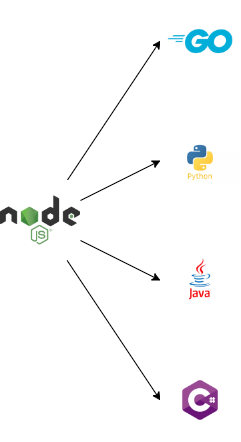
\includegraphics[height = 3cm]{pictures/DaNgonNgu/_DaNgonNgu.png}

% \caption{ViDuHinhAnhTheoChieuDoc}

\end{figure}

% Thêm vào hình SQL riêng